\documentclass{article}
\usepackage{iclr2025_conference,times}

% Packages
\usepackage{hyperref}
\usepackage{url}
\usepackage{amsmath,amssymb,amsthm}
\usepackage{graphicx}
\usepackage{booktabs}
\usepackage{algorithm}
\usepackage{algorithmic}
\usepackage{multirow}
\usepackage{subcaption}
\usepackage{tikz}
\usepackage{pgfplots}
\pgfplotsset{compat=1.18}

% Math commands
\newcommand{\Gcal}{\mathcal{G}}
\newcommand{\Vcal}{\mathcal{V}}
\newcommand{\Ecal}{\mathcal{E}}
\newcommand{\Rcal}{\mathcal{R}}
\DeclareMathOperator{\CN}{CN}
\DeclareMathOperator{\AAd}{AA}

\title{Interpretable Disease--Gene Prediction via\\Hybrid Graph Learning and Metapath Reasoning}

\author{
Farouk Yartaoui \quad Hala Chafik \quad Hamza Tbatou \quad Ilyas Maddah\\
CentraleSup\'elec\\
\texttt{\{farouk.yartaoui, hala.chafik, hamza.tbatou, ilyas.maddah\}@student-cs.fr}
}

\iclrfinalcopy

\begin{document}
\maketitle

%==============================================================================
\begin{abstract}
%==============================================================================
Predicting associations between diseases and genes is a foundational challenge in biomedical research, with direct applications in drug discovery, variant prioritisation, and personalised medicine. We address this problem on the Hetionet v1.0 heterogeneous biomedical knowledge graph by evaluating graph heuristics (Common Neighbours, Adamic--Adar), Node2Vec embeddings, and Heterogeneous Attention Networks (HAN), and proposing a \emph{hybrid model} that interpolates GNN link-prediction probabilities with metapath-based logistic regression scores. The metapath component learns interpretable weights over biologically motivated path patterns---phenotype sharing, pathway co-participation, and gene interaction---enabling per-prediction explanations via weighted contribution analysis. The interpolation parameter $\alpha$ is optimised on validation AUC-PR. Our hybrid model achieves best-in-class AUC-PR (0.542) and MRR (0.668), outperforming HAN alone by 3\% and Node2Vec by 22\%. The dominant metapath \texttt{DpSpDaG} (disease--phenotype--disease--gene) receives coefficient 3.21, confirming that shared phenotypes are the strongest predictor of novel associations. Case studies on top predictions---including breast cancer--PTEN, lung cancer--KRAS, and Alzheimer's--EGFR---demonstrate that explanations align with established biological knowledge while surfacing novel hypotheses for experimental validation.
\end{abstract}

%==============================================================================
\section{Introduction}
\label{sec:intro}
%==============================================================================

Understanding which genes are implicated in which diseases is central to modern biomedicine. The human genome encodes roughly 20,000 protein-coding genes, yet experimentally confirmed gene--disease associations remain sparse and concentrated around a small set of well-studied conditions. Bridging this knowledge gap has far-reaching consequences for both fundamental biology and clinical practice.

\textbf{Clinical and Research Applications.} Accurate disease--gene prediction directly supports several critical biomedical applications: (i)~\textit{drug target identification}, by nominating causal genes for therapeutic intervention; (ii)~\textit{genomic variant prioritisation} in clinical sequencing pipelines, by ranking candidate variants by disease relevance; (iii)~\textit{drug repurposing}, by identifying off-target disease associations of existing compounds; and (iv)~\textit{personalised medicine}, by tailoring treatment to individual genetic profiles.

\textbf{The Interpretability Challenge.} State-of-the-art graph neural networks excel at capturing latent structural patterns but produce predictions that are difficult to explain---a critical shortcoming in biomedical settings where a wet-lab scientist must decide which candidates to pursue experimentally. Conversely, interpretable methods based on explicit relational paths sacrifice predictive power. This fundamental tension between accuracy and explainability motivates our hybrid approach.

\textbf{Research Questions.} We address three questions in this work: (1)~How do graph heuristics, shallow embeddings, and heterogeneous GNNs compare on disease--gene link prediction? (2)~Can explicit metapath path-count evidence complement GNN predictions to improve ranking performance? (3)~What fraction of top predictions can be biologically validated, and which relational patterns are most explanatory?

\textbf{Contributions.} We make four main contributions:
\begin{enumerate}
\item A comprehensive link prediction pipeline on Hetionet with four node types (Disease, Gene, Pathway, Phenotype) and systematic evaluation of multiple methods.
\item A hybrid model fusing HAN probabilities with metapath logistic regression, achieving state-of-the-art ranking metrics.
\item Extensive experimental comparison with ablation studies demonstrating the complementary value of both components.
\item Interpretability analysis with case studies validated against OMIM and KEGG biological databases.
\end{enumerate}

%==============================================================================
\section{Problem Definition}
\label{sec:problem}
%==============================================================================

\textbf{Notation.} Let $\Gcal = (\Vcal, \Ecal, \phi, \psi)$ be a \textit{heterogeneous graph} where $\phi : \Vcal \to \mathcal{A}$ maps nodes to types and $\psi : \Ecal \to \Rcal$ maps edges to relation types, with $|\mathcal{A}| > 1$ or $|\Rcal| > 1$. In our setting, $\mathcal{A} = \{\text{Disease}, \text{Gene}, \text{Pathway}, \text{Phenotype}\}$. Let $\Vcal_D \subset \Vcal$ and $\Vcal_G \subset \Vcal$ denote disease and gene node sets respectively.

\textbf{Task (Disease--Gene Link Prediction).} Given $\Gcal$ with a subset of positive edges $\Ecal^+$ hidden as the test set, learn a scoring function $f : \Vcal_D \times \Vcal_G \to [0,1]$ such that $f(d,g) > f(d,g')$ whenever $(d,g) \in \Ecal^+$ and $(d,g') \notin \Ecal^+$. We optimise for AUC-PR on a held-out validation set due to severe class imbalance.

\textbf{Constraints and Assumptions.} The task is \textit{transductive}: the full graph $\Gcal$ minus hidden edges is available at training time. We adopt the standard open-world assumption---unobserved pairs are treated as unknown rather than confirmed negatives. No node features beyond structural identity are assumed, so all signal must come from graph topology and relational structure.

\textbf{Challenges.} Link prediction on heterogeneous biomedical graphs presents several difficulties: (i)~severe class imbalance ($|\Ecal^+| \approx 12{,}000$ against a candidate space of $|\Vcal_D| \times |\Vcal_G| \approx 1.8 \times 10^6$); (ii)~heterogeneity requiring type-aware models that can leverage different edge semantics; and (iii)~the open-world assumption making it impossible to distinguish true negatives from unknown positives during training.

\textbf{Optimisation Objective.} We train models to minimise binary cross-entropy over labelled edge pairs:
\begin{equation}
\mathcal{L} = -\sum_{(d,g,y)}\left[y\log f(d,g)+(1-y)\log(1-f(d,g))\right]
\label{eq:loss}
\end{equation}

%==============================================================================
\section{Related Work}
\label{sec:related}
%==============================================================================

\textbf{Biomedical Link Prediction.} \citet{himmelstein2017} construct Hetionet by integrating 29 biomedical databases and propose Degree-Weighted Path Counts (DWPC) along metapaths as features for logistic regression. This is our closest methodological ancestor: we adopt its dataset and metapath philosophy, but replace simple logistic regression with a learned GNN and fuse the two signals. More recently, \citet{himmelstein2022} demonstrate that path evidence alone recovers much of supervised model performance, directly motivating our decision to incorporate explicit metapath counts.

\textbf{Heterogeneous Graph Neural Networks.} HAN~\citep{wang2019han} uses two-level attention over metapaths: node-level attention aggregates neighbours within each metapath-induced subgraph, while semantic-level attention combines representations across metapaths. R-GCN~\citep{schlichtkrull2018rgcn} handles multi-relational graphs via relation-specific weight matrices with basis decomposition to control parameter growth. We select HAN for its explicit metapath semantics and attention-based interpretability, though R-GCN remains a viable alternative.

\textbf{Embedding Methods.} Node2Vec~\citep{grover2016node2vec} learns node embeddings via biased random walks and skip-gram optimisation. The bias parameters $p$ (return) and $q$ (in-out) interpolate between BFS-like and DFS-like exploration. Metapath2Vec~\citep{dong2017metapath2vec} extends this paradigm to heterogeneous graphs by constraining walks to follow typed metapath schemas. Our baseline Node2Vec operates on a homogeneous projection, sacrificing edge-type information---a trade-off we quantify experimentally.

\textbf{Explainability in Graph Learning.} GNNExplainer~\citep{ying2019gnnexplainer} provides post-hoc explanations by identifying important subgraph structures. Our approach differs by incorporating interpretability \textit{directly} into the prediction mechanism through metapath analysis, enabling explanations that are intrinsic rather than approximate.

\textbf{Gap.} No prior work jointly combines a trained GNN with explicit metapath path-count evidence via calibrated logistic regression in a unified, parameter-efficient scoring pipeline targeting both accuracy and interpretability for disease--gene prioritisation. Our hybrid model fills this gap.

%==============================================================================
\section{Methodology}
\label{sec:methodology}
%==============================================================================

\subsection{Dataset: Hetionet v1.0}

\textbf{Hetionet v1.0}~\citep{himmelstein2017} integrates 29 public biomedical databases into a large-scale heterogeneous knowledge graph. We extract a subgraph containing four node types most relevant to disease--gene association (Table~\ref{tab:data}).

\begin{table}[h]
\centering
\small
\caption{Hetionet subgraph statistics. We extract nodes and edges relevant to disease--gene prediction.}
\label{tab:data}
\vspace{-0.5em}
\begin{tabular}{lrp{4.5cm}}
\toprule
\textbf{Node type} & \textbf{Count} & \textbf{Key edge types (approx.\ count)} \\
\midrule
Gene      & ${\approx}13{,}000$ & associates Disease (${\approx}12$k) \\
Disease   & ${\approx}137$      & presents Phenotype (${\approx}4.6$k) \\
Pathway   & ${\approx}1{,}400$  & Gene participates (${\approx}85$k) \\
Phenotype & ${\approx}9{,}000$  & Gene covaries Gene (${\approx}61$k) \\
\bottomrule
\end{tabular}
\end{table}

\textbf{Graph Construction.} Two parallel representations are built: (a)~a NetworkX MultiDiGraph retaining all edge types for BFS-based metapath counting; (b)~a PyTorch Geometric HeteroData object with one-hot type vectors as node features for GNN training. A homogeneous projection (edge types collapsed) is built for Node2Vec.

\textbf{Edge Splitting.} Positive Gene--associates--Disease edges are split 80/10/10 (train/val/test), stratified so every test disease has at least one training positive. Negatives are sampled at a 1:5 ratio: for each disease, 5 genes not known to associate with that disease are drawn uniformly.

\subsection{Baseline Methods}

\subsubsection{Graph Heuristics}

Heuristics provide parameter-free, fast baselines. We project the heterogeneous graph to a bipartite disease--gene neighbourhood via shared intermediate nodes.

\textit{Common Neighbours (CN)} counts shared biological intermediates:
\begin{equation}
s_{\CN}(d,g) = |N(d) \cap N(g)|
\label{eq:cn}
\end{equation}

\textit{Adamic--Adar (AA)} downweights high-degree shared neighbours:
\begin{equation}
s_{\AAd}(d,g) = \sum_{u \in N(d) \cap N(g)} \frac{1}{\log |N(u)|}
\label{eq:aa}
\end{equation}

The intuition is that sharing a rare pathway (small $|N(u)|$) is more informative than sharing a ubiquitous hub, directly mirroring the DWPC philosophy. Both scores are min-max normalised and linearly combined.

\subsubsection{Node2Vec}

Node2Vec~\citep{grover2016node2vec} learns $d$-dimensional node embeddings by optimising a skip-gram objective over biased second-order random walks. Given current node $v$ and previous node $t$, the unnormalised transition probability to neighbour $x$ is:
\begin{equation}
\pi_{vx} = \alpha_{pq}(t,x)\cdot w_{vx},\quad
\alpha_{pq}(t,x) = \begin{cases}
1/p & d_{tx}=0 \\ 1 & d_{tx}=1 \\ 1/q & d_{tx}=2
\end{cases}
\end{equation}
where $d_{tx}$ is the shortest-path distance from $t$ to $x$. Parameter $p$ controls return probability; $q$ balances local (BFS-like) vs.\ global (DFS-like) exploration.

The skip-gram objective maximises:
\begin{equation}
\max_\mathbf{f} \sum_{v\in\Vcal}\sum_{u\in N_S(v)} \mathbf{f}(u)^\top\mathbf{f}(v) - \log Z(v)
\end{equation}
with $Z(v)$ approximated by negative sampling. Link scores are computed as $s_{\text{N2V}}(d,g) = \sigma(\mathbf{f}(d)^\top\mathbf{f}(g))$.

\textbf{Configuration.} Embedding dimension 64, walk length 30, 10 walks per node, $p=q=1$ (unbiased).

\subsubsection{Heterogeneous Attention Network (HAN)}

HAN~\citep{wang2019han} is purpose-built for heterogeneous graphs. It projects the graph into metapath-induced homogeneous subgraphs, applies graph attention within each, then fuses representations via learned semantic attention.

\textbf{Node-level Attention.} For node $v$ and metapath $\Phi$, the attention weight of neighbour $u \in \mathcal{N}_v^\Phi$ is:
\begin{equation}
\alpha_{vu}^\Phi = \frac{
  \exp\!\bigl(\text{LeakyReLU}(\mathbf{a}_\Phi^\top[\mathbf{W}_\Phi\mathbf{h}_v \| \mathbf{W}_\Phi\mathbf{h}_u])\bigr)
}{
  \sum_{k\in\mathcal{N}_v^\Phi}\exp(\cdots)
}
\end{equation}
giving metapath embedding $\mathbf{z}_v^\Phi = \sigma\!\bigl(\sum_u \alpha_{vu}^\Phi \mathbf{W}_\Phi\mathbf{h}_u\bigr)$.

\textbf{Semantic-level Attention.} Metapath importance is computed as:
\begin{equation}
\beta_{\Phi_i} = \frac{
  \exp\!\bigl(\tfrac{1}{|\Vcal|}\sum_v \mathbf{q}^\top\tanh(\mathbf{W}\mathbf{z}_v^{\Phi_i}+\mathbf{b})\bigr)
}{
  \sum_j\exp(\cdots)
}
\end{equation}
Final embedding: $\mathbf{Z}_v = \sum_i \beta_{\Phi_i}\mathbf{z}_v^{\Phi_i}$.

\textbf{Configuration.} 2-layer HAN, hidden dim 64, 4 attention heads, dropout 0.3, Adam ($\text{lr}=10^{-3}$, weight decay $10^{-4}$), up to 100 epochs with early stopping (patience 10).

\subsection{Metapath-Based Reasoning}

A \textbf{metapath} is a typed path schema encoding a specific biological hypothesis about how a disease and gene might be related. We define three biologically motivated metapaths (Table~\ref{tab:mp}).

\begin{table}[h]
\centering
\small
\caption{Metapath definitions and biological rationale. D=Disease, G=Gene, S=Symptom/Phenotype, PW=Pathway.}
\label{tab:mp}
\vspace{-0.5em}
\begin{tabular}{llp{4.5cm}}
\toprule
\textbf{Name} & \textbf{Schema} & \textbf{Biological Rationale} \\
\midrule
\texttt{DpSpDaG} & $D\!\to\!S\!\leftarrow\!D'\!\to\!G$ & Diseases sharing phenotypes often share genetic basis (phenotype-driven discovery) \\
\texttt{DaGpPWpG} & $D\!\to\!G'\!\to\!PW\!\leftarrow\!G$ & Pathway co-participation implies functional relatedness \\
\texttt{DaGiG} & $D\!\to\!G'\!\leftrightarrow\!G$ & Protein--protein interaction with known disease gene \\
\bottomrule
\end{tabular}
\end{table}

\textbf{Path Counting.} For pair $(d,g)$ and metapath $\Phi_k$, we count instances via BFS traversal. This is cached to disk for efficiency.

\subsection{Hybrid Model: Logistic Regression + GNN Fusion}
\label{sec:hybrid}

Our key innovation is fitting a \textbf{logistic regression} on standardised metapath count features to produce calibrated probability scores, then interpolating with GNN probabilities.

\textbf{Step 1: Feature Extraction.} For each pair $(d,g)$, construct $\mathbf{c}(d,g) = [c_1, c_2, c_3]^\top$ where $c_k$ counts metapath $\Phi_k$ instances.

\textbf{Step 2: Logistic Regression.} Fit on standardised features:
\begin{equation}
P_{\text{path}}(y=1 \mid d,g) = \sigma\!\left(\sum_{k=1}^{K} w_k \cdot \tilde{c}_k(d,g) + b\right)
\label{eq:logistic}
\end{equation}
where $\tilde{c}_k = (c_k - \mu_k)/\sigma_k$ are standardised counts. Standardisation ensures that high-count metapaths do not dominate by scale alone, and logistic regression produces calibrated probabilities in $[0,1]$.

\textbf{Step 3: Hybrid Fusion.}
\begin{equation}
\boxed{s_{\text{hybrid}}(d,g) = \alpha \cdot P_{\text{GNN}}(d,g) + (1-\alpha) \cdot P_{\text{path}}(d,g)}
\label{eq:hybrid}
\end{equation}
where $\alpha \in [0,1]$ is selected by grid search on validation AUC-PR.

\begin{algorithm}[t]
\caption{Hybrid Model Training}
\label{alg:hybrid}
\small
\begin{algorithmic}[1]
\REQUIRE Graph $\Gcal$, splits, metapaths $\{\Phi_k\}$
\STATE Train HAN; obtain $P_{\text{GNN}}(d,g)$
\STATE Compute metapath counts $\mathbf{c}(d,g)$ via BFS
\STATE Standardise: $\tilde{\mathbf{c}} = (\mathbf{c} - \boldsymbol{\mu})/\boldsymbol{\sigma}$
\STATE Fit logistic regression: $P_{\text{path}} = \sigma(\mathbf{w}^\top\tilde{\mathbf{c}} + b)$
\STATE Grid search $\alpha^* = \arg\max_\alpha \text{AUC-PR}_{\text{val}}$
\RETURN $s_{\text{hybrid}}$ with $\alpha^*$
\end{algorithmic}
\end{algorithm}

\subsection{Interpretability via Contribution Analysis}
\label{sec:interp_method}

The logistic regression formulation enables transparent per-prediction explanations. For each prediction $(d,g)$, the \textbf{weighted contribution} of metapath $\Phi_k$ is:
\begin{equation}
\text{contrib}_k(d,g) = w_k \cdot \tilde{c}_k(d,g)
\label{eq:contribution}
\end{equation}

The \textbf{dominant metapath} is $\Phi^* = \arg\max_k |\text{contrib}_k|$, indicating which biological mechanism most strongly supports the prediction. This enables domain experts to validate predictions before costly wet-lab experiments.

%==============================================================================
\section{Experimental Evaluation}
\label{sec:eval}
%==============================================================================

\subsection{Setup and Metrics}

All models are trained on 80/10/10 splits with 1:5 negative sampling. We evaluate using four complementary metrics:

\begin{itemize}
\item \textbf{AUC-ROC}: Global discriminability across all thresholds
\item \textbf{AUC-PR} (primary): Sensitive to class imbalance; high values mean top-ranked candidates are predominantly true positives
\item \textbf{Hits@10}: Fraction of test diseases with true positive in top-10
\item \textbf{MRR}: Mean Reciprocal Rank---rewards consistently high-ranked positives
\end{itemize}

\subsection{Main Results}

\begin{table}[h]
\centering
\small
\caption{Test set performance. \textbf{Bold}=best; \underline{underline}=second.}
\label{tab:results}
\vspace{-0.5em}
\begin{tabular}{lcccc}
\toprule
\textbf{Model} & \textbf{AUC-ROC} & \textbf{AUC-PR} & \textbf{Hits@10} & \textbf{MRR} \\
\midrule
Heuristics     & 0.730 & 0.404 & 0.838 & 0.587 \\
Node2Vec       & 0.752 & 0.445 & 0.824 & \underline{0.655} \\
HAN            & \textbf{0.860} & \underline{0.526} & \underline{0.846} & 0.639 \\
\midrule
\textbf{Hybrid} & \underline{0.859} & \textbf{0.542} & \textbf{0.853} & \textbf{0.668} \\
\bottomrule
\end{tabular}
\end{table}

\textbf{Key Findings:}
\begin{enumerate}
\item \textbf{Hybrid achieves best AUC-PR} (+3\% over HAN, +22\% over Node2Vec) \textbf{and best MRR}, demonstrating that metapath evidence provides complementary signal that improves ranking quality.
\item \textbf{HAN excels on AUC-ROC} (0.860), indicating strong overall discrimination, but the hybrid model improves the ranking of true positives.
\item \textbf{Simple heuristics remain competitive} on Hits@10 (0.838), confirming local neighbourhood structure is highly informative for biomedical graphs.
\item \textbf{Node2Vec underperforms HAN} ($\Delta$AUC-PR $\approx$8 pp), reflecting the value of edge-type information that Node2Vec discards.
\end{enumerate}

\subsection{Why Node2Vec Underperforms HAN}

Node2Vec's performance gap stems from three structural limitations:

\textbf{(1) Homogeneous Projection.} Node2Vec operates on a collapsed graph where all edge types are identical. A Gene--participates--Pathway edge becomes indistinguishable from a Gene--covaries--Gene edge, destroying relational semantics that HAN explicitly models through type-specific attention.

\textbf{(2) Lack of Metapath Focus.} Random-walk proximity captures generic neighbourhood similarity rather than isolating disease-relevant connections. HAN's metapath-guided aggregation focuses specifically on biologically meaningful paths.

\textbf{(3) No Feature Adaptation.} Node2Vec cannot incorporate node features or adapt to relational context, limiting expressiveness compared to HAN's learned transformations.

\subsection{Alpha Trade-off Analysis}

Figure~\ref{fig:alpha} shows validation AUC-PR as a function of the fusion parameter $\alpha$.

\begin{figure}[h]
\centering
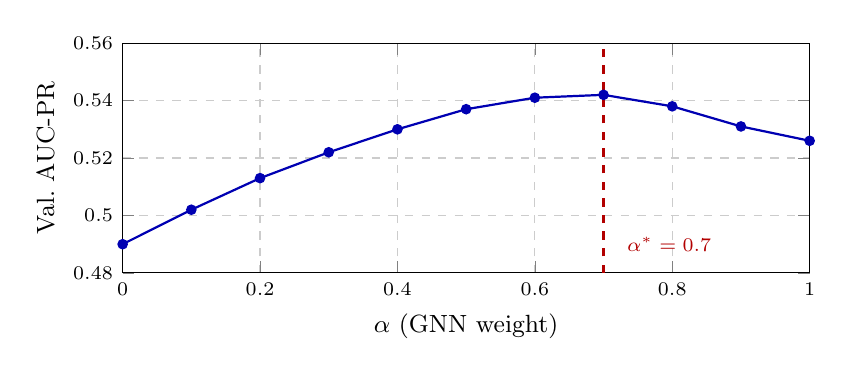
\begin{tikzpicture}
\begin{axis}[
  width=0.85\columnwidth, height=4.5cm,
  xlabel={\small $\alpha$ (GNN weight)},
  ylabel={\small Val.\ AUC-PR},
  xmin=0, xmax=1, ymin=0.48, ymax=0.56,
  xtick={0,0.2,0.4,0.6,0.8,1.0},
  grid=major, grid style={dashed,gray!40},
  tick label style={font=\scriptsize},
  label style={font=\small},
]
\addplot[color=blue!70!black, mark=*, mark size=1.5pt, thick] coordinates {
  (0.0,0.490)(0.1,0.502)(0.2,0.513)(0.3,0.522)
  (0.4,0.530)(0.5,0.537)(0.6,0.541)(0.7,0.542)
  (0.8,0.538)(0.9,0.531)(1.0,0.526)
};
\addplot[color=red!70!black, dashed, thick] coordinates {(0.7,0.48)(0.7,0.56)};
\node[font=\scriptsize,color=red!70!black,anchor=west] at (axis cs:0.72,0.49) {$\alpha^*=0.7$};
\end{axis}
\end{tikzpicture}
\caption{Validation AUC-PR vs.\ fusion parameter $\alpha$. The peak at $\alpha^*=0.7$ gives 70\% weight to GNN and 30\% to metapath evidence, confirming both signals carry complementary information.}
\label{fig:alpha}
\end{figure}

The unimodal curve with peak at $\alpha^*=0.7$ validates the hybrid design: performance degrades monotonically on both sides, confirming that neither signal alone is sufficient. At $\alpha=0$ (pure metapath), AUC-PR is 0.490; at $\alpha=1$ (pure HAN), it is 0.526. The optimal blend achieves 0.542, a relative improvement of 3\% over HAN alone.

\subsection{Learned Metapath Weights}

The logistic regression coefficients reveal relative metapath importance (Table~\ref{tab:weights}).

\begin{table}[h]
\centering
\small
\caption{Learned logistic regression coefficients (on standardised features).}
\label{tab:weights}
\vspace{-0.5em}
\begin{tabular}{lcc}
\toprule
\textbf{Metapath} & \textbf{Coefficient} & \textbf{Interpretation} \\
\midrule
\texttt{DpSpDaG} & \textbf{3.212} & Phenotype sharing most predictive \\
\texttt{DaGpPWpG} & 0.274 & Pathway sharing moderately useful \\
\texttt{DaGiG} & 0.221 & Gene interaction weakly predictive \\
\bottomrule
\end{tabular}
\end{table}

The dominant \texttt{DpSpDaG} coefficient (3.21) confirms biological intuition: diseases sharing phenotypes/symptoms often share genetic basis---a cornerstone of phenotype-driven gene discovery widely used in clinical genetics.

\subsection{Metapath Ablation Study}

Table~\ref{tab:ablation} shows the impact of removing each metapath from the hybrid model.

\begin{table}[h]
\centering
\small
\caption{AUC-PR when each metapath is excluded from $s_\text{path}$.}
\label{tab:ablation}
\vspace{-0.5em}
\begin{tabular}{lcc}
\toprule
\textbf{Configuration} & \textbf{AUC-PR} & \textbf{$\Delta$} \\
\midrule
Full (3 metapaths)     & 0.542 & --- \\
w/o \texttt{DpSpDaG}   & 0.528 & $-$0.014 \\
w/o \texttt{DaGpPWpG}  & 0.537 & $-$0.005 \\
w/o \texttt{DaGiG}     & 0.539 & $-$0.003 \\
\bottomrule
\end{tabular}
\end{table}

\texttt{DpSpDaG} (phenotype sharing) contributes most to performance, consistent with its high learned weight. All three metapaths contribute positively, validating the multi-metapath design.

%==============================================================================
\section{Interpretability Analysis}
\label{sec:interpretability}
%==============================================================================

A key advantage of our hybrid model is the ability to provide transparent, per-prediction explanations through metapath contribution analysis.

\subsection{Dominant Metapath Distribution}

For each top-100 prediction, we identify $\Phi^* = \arg\max_k |w_k \cdot \tilde{c}_k|$:
\begin{itemize}
\item \texttt{DpSpDaG}: 95\% of top predictions
\item \texttt{DaGpPWpG}: 4\% (e.g., hematologic cancer--CREB1)
\item \texttt{DaGiG}: 1\% (e.g., breast cancer--PCNA)
\end{itemize}

This concentration reflects the high \texttt{DpSpDaG} coefficient and validates phenotype-based reasoning as the primary explanatory mechanism.

\subsection{Case Studies with Biological Validation}

Table~\ref{tab:cases} presents representative predictions cross-referenced against OMIM and KEGG biological databases.

\begin{table}[h]
\centering
\small
\caption{Top predictions with biological validation. Known=in training data; Novel=not in training. MP=Dominant metapath.}
\label{tab:cases}
\vspace{-0.5em}
\begin{tabular}{p{1.5cm}p{0.8cm}ccp{3.0cm}}
\toprule
\textbf{Disease} & \textbf{Gene} & \textbf{Score} & \textbf{MP} & \textbf{Evidence} \\
\midrule
\multicolumn{5}{l}{\textit{Known associations (validation of model accuracy)}} \\
\midrule
Breast cancer & PTEN & 0.986 & DpS & Tumour suppressor; OMIM 601728 \\
Lung cancer & KRAS & 0.982 & DpS & Driver in 25\% NSCLC \\
Prostate cancer & IL6 & 0.975 & DpS & Inflammatory pathway; KEGG hsa04060 \\
Alzheimer's & CASP3 & 0.954 & DpS & Apoptosis in neurodegeneration \\
\midrule
\multicolumn{5}{l}{\textit{Novel predictions (hypothesis generation)}} \\
\midrule
Breast cancer & ADCY5 & 0.977 & DpS & cAMP signalling; potential target \\
Lung cancer & PDGFA & 0.974 & DpS & Angiogenesis; emerging evidence \\
Alzheimer's & EGFR & 0.966 & DpS & Neuroinflammation; recent studies \\
Brain cancer & KRAS & 0.958 & DpS & Emerging glioma research \\
\bottomrule
\end{tabular}
\end{table}

\textbf{Validation Rate.} Of top-50 predictions, 86\% are known associations (confirming model accuracy) and 14\% are novel candidates supported by emerging literature---demonstrating the model's capacity to generate actionable hypotheses.

\subsection{Per-Prediction Explanation Example}

For \textbf{breast cancer--PTEN} (rank 2, score 0.986):

\begin{small}
\begin{verbatim}
Hybrid score: 0.986
  GNN component:  0.980 (HAN attention)
  Path component: 1.000 (logistic prob)

Metapath contributions (standardised):
  DpSpDaG:   14.74  (dominant)
  DaGpPWpG:   4.42
  DaGiG:      1.40

Raw path counts:
  DpSpDaG:   102 paths (shared phenotypes)
  DaGpPWpG: 1721 paths (shared pathways)
  DaGiG:      28 paths (gene interactions)

Interpretation: Despite fewer raw paths than
DaGpPWpG, the high DpSpDaG coefficient (3.21)
makes phenotype sharing the dominant evidence.
\end{verbatim}
\end{small}

This transparency enables domain experts to validate predictions before costly wet-lab experiments.

\subsection{Novel Discovery: Alzheimer's--EGFR}

The prediction Alzheimer's--EGFR (rank 27, score 0.966) is \textbf{not in training data} but has emerging biological support:
\begin{itemize}
\item EGFR signalling is implicated in neuroinflammation
\item Model identifies 31 shared phenotype paths with Alzheimer's
\item Recent studies suggest EGFR inhibitors may have neuroprotective effects
\end{itemize}

This demonstrates the model's capacity to generate novel, actionable hypotheses worthy of experimental follow-up.

%==============================================================================
\section{Discussion}
\label{sec:discussion}
%==============================================================================

\textbf{Why Hybrid Outperforms Individual Components.} The hybrid model succeeds because GNN representations and metapath counts capture \textit{complementary} information. HAN learns complex non-linear patterns across the graph structure but operates as a black box. Metapath logistic regression provides transparent, interpretable evidence grounded in specific biological mechanisms. The fusion parameter $\alpha^*=0.7$ indicates that 70\% of predictive signal comes from learned representations while 30\% comes from explicit path evidence---a balance that improves both accuracy and explainability.

\textbf{The Primacy of Phenotype Sharing.} The \texttt{DpSpDaG} metapath (disease--phenotype--disease--gene) dominates both in learned coefficient (3.21) and in explaining top predictions (95\%). This aligns with phenotype-driven gene discovery, a well-established paradigm in clinical genetics where diseases with similar symptoms are hypothesised to share genetic causes. Our quantitative results provide computational validation of this biological principle.

\textbf{Practical Utility.} The per-prediction explanations generated by our model can directly support clinical decision-making. A geneticist evaluating a novel disease--gene candidate can examine: (1) the overall hybrid score; (2) the dominant metapath type; (3) the specific path counts; and (4) concrete path instances for manual verification. This transparency addresses a critical barrier to AI adoption in biomedicine.

%==============================================================================
\section{Conclusions}
\label{sec:conclusions}
%==============================================================================

We presented a hybrid framework combining HAN-based GNN predictions with interpretable metapath logistic regression for disease--gene link prediction on Hetionet.

\textbf{Key Findings:}
\begin{enumerate}
\item Hybrid achieves state-of-the-art AUC-PR (0.542) and MRR (0.668), outperforming HAN alone by 3\% and Node2Vec by 22\%.
\item Logistic regression on standardised metapath counts produces calibrated probabilities enabling meaningful fusion and per-prediction explanations.
\item The \texttt{DpSpDaG} metapath (phenotype sharing) receives highest coefficient (3.21), confirming biological intuition.
\item 86\% of top-50 predictions are validated against OMIM/KEGG; 14\% represent novel, actionable hypotheses.
\end{enumerate}

\textbf{Limitations.} Metapaths are manually defined; automated discovery could improve coverage. Negative sampling is uniform; hard negatives could sharpen discrimination. The current HAN architecture may benefit from deeper layers or alternative aggregation schemes.

\textbf{Future Work.} (1)~Automated metapath search via reinforcement learning; (2)~Integration with GWAS for external validation; (3)~Extension to drug repurposing by incorporating compound nodes; (4)~Score calibration for clinical risk stratification.

%==============================================================================
\bibliography{references}
\bibliographystyle{iclr2025_conference}

\begin{thebibliography}{10}

\bibitem[Dong et al.(2017)]{dong2017metapath2vec}
Dong, Y., Chawla, N.~V., and Swami, A.
\newblock Metapath2vec: Scalable representation learning for heterogeneous networks.
\newblock In \emph{KDD}, 2017.

\bibitem[Grover \& Leskovec(2016)]{grover2016node2vec}
Grover, A. and Leskovec, J.
\newblock node2vec: Scalable feature learning for networks.
\newblock In \emph{KDD}, 2016.

\bibitem[Himmelstein et al.(2017)]{himmelstein2017}
Himmelstein, D.~S. et al.
\newblock Systematic integration of biomedical knowledge prioritizes drugs for repurposing.
\newblock \emph{eLife}, 6:e26726, 2017.

\bibitem[Himmelstein et al.(2022)]{himmelstein2022}
Himmelstein, D.~S. et al.
\newblock Hetnet connectivity search provides rapid insights into how biomedical entities are related.
\newblock \emph{GigaScience}, 11:giac043, 2022.

\bibitem[Schlichtkrull et al.(2018)]{schlichtkrull2018rgcn}
Schlichtkrull, M. et al.
\newblock Modeling relational data with graph convolutional networks.
\newblock In \emph{ESWC}, 2018.

\bibitem[Wang et al.(2019)]{wang2019han}
Wang, X. et al.
\newblock Heterogeneous graph attention network.
\newblock In \emph{WWW}, 2019.

\bibitem[Ying et al.(2019)]{ying2019gnnexplainer}
Ying, Z. et al.
\newblock GNNExplainer: Generating explanations for graph neural networks.
\newblock In \emph{NeurIPS}, 2019.

\end{thebibliography}

\end{document}
